%%% Ne pas modifier jusqu'à la ligne 25
\documentclass[a4paper,12pt]{book}
\usepackage[utf8]{inputenc}
\usepackage[french]{babel}
%%\usepackage{CJK}
\usepackage{yhmath}
\usepackage[left=2cm,right=2cm,top=3cm,bottom=2cm, headheight=1.5cm,headsep=1.5cm]{geometry}
%%\usepackage{CJKutf8}
\usepackage{amsfonts}
\usepackage{amsmath,amsfonts,amssymb,dsfont}
\usepackage{graphicx}
\usepackage{enumitem}		%\enumerate-resume
\usepackage[colorlinks=true,unicode={true},hyperindex=false, linkcolor=blue, urlcolor=blue]{hyperref}
\newcommand{\myref}[1]{\ref{#1} page \pageref{#1}}

\addto\captionsfrench{\def\tablename{Tableau}}  %légendes des tableaux
\renewcommand\thesection{\Roman{section}~-~} 
\renewcommand\thesubsection{\Roman{section}.\Alph{subsection}~-~} 
\renewcommand\thesubsubsection{\Roman{section}.\Alph{subsection}.\arabic{subsubsection}~-~} 

\newcommand{\conclusion}[1]{\newline \centerline{\fbox{#1}}}

\setcounter{secnumdepth}{3}
\parindent=0pt

\usepackage{fancyhdr}
\pagestyle{fancy}

\lhead{SJTU-ParisTech} 
%%%%%%%%%%%%%%%%%%%%%%%%%%%%%%%%%%
\chead{DM5}
\rhead{Daniel 518261910024}

\begin{document}
\renewcommand{\labelitemi}{$\blacktriangleright$}
\renewcommand{\labelitemii}{$\bullet$}


\section{Détermination expérimentale d’une enthalpie de réaction}
\begin{figure}[h]
    \begin{center}
    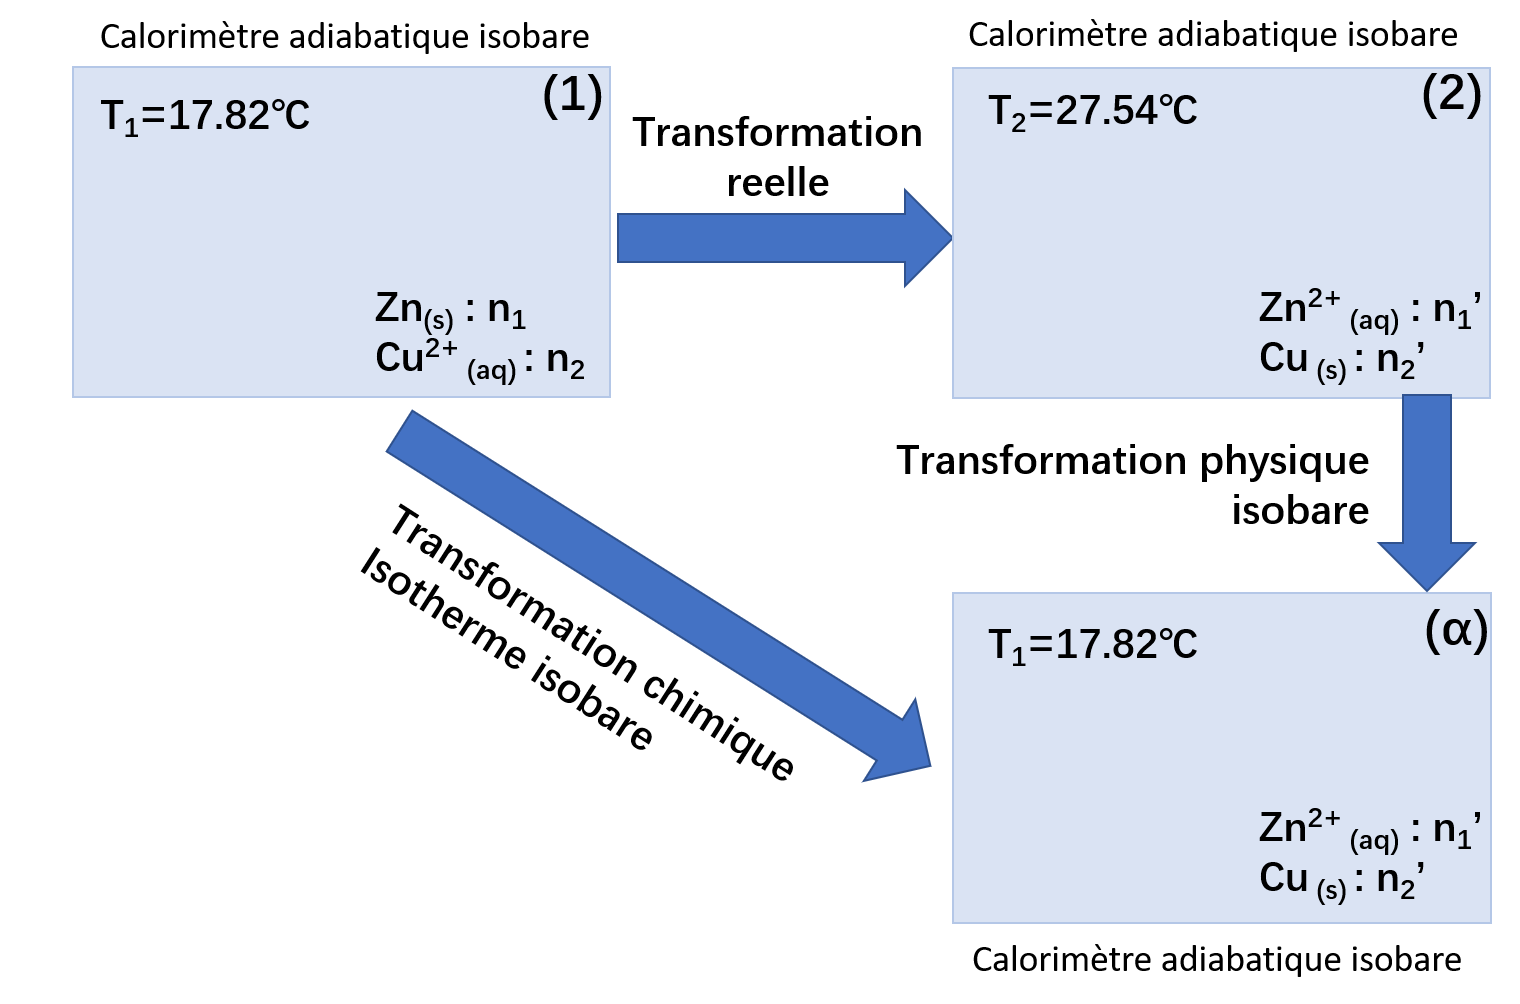
\includegraphics[scale=0.6]{dm5.png}
    \end{center}
    \caption{Figure du système étudié}
\end{figure}
\subsection{}

\begin{table}[h]
\begin{center}
    \begin{tabular}{l|ccccccc}
    \hline
                      & $Zn_{(s)}$      & + & $Cu_{(aq)}^{2+}$       & = & $Cu_{(s)}$ & + & $Zn_{(aq)}^{2+}$ \\ \hline
        $n_{initial}$ & $n_{1}$       &   & $n_{2}$      &   & $0$ & & $0$\\ 
        $n_{final}$      & $n_{1}-2\xi_{max}$  &   & $n_{2}-\xi_{max}$  &   & $\xi_{max}$ & & $\xi_{max}$\\ 
    \end{tabular}
\end{center}
\end{table}
On a $n_1=\frac{m_{Zn}}{M_{Zn}}=\frac{3.2}{65.4}=0.049\,mol$, et $n_2=V*c=150*0.200=3.00*10^{-2}\,mol$, donc $\xi_{max}=n_2=0.03\,mol$

\hspace*{\fill} 

Car c'est une tranformation isobare est adiabatique, on a $\Delta H_{1 \to 2}=Q_{recue}=0$

\hspace*{\fill} 

On va donc introduit un état fictif $(\alpha)$, et on va séparer la transformation par deux étapes fictives.

\begin{itemize}
    \item $(1) \to (\alpha)$: On a $\Delta H_{1 \to \alpha}=\Delta H_{1 \to \alpha}^\circ$ puisque l'enthalpie est 
          indépendante de la pression, est 
          
          \hspace*{\fill} 

          c'est une tranformation isotherme isobare. 
          
          \hspace*{\fill} 

          On a alors $\Delta H_{1 \to \alpha}=(\xi_{max}-\xi_{in})\Delta_rH^\circ=\xi_{max}\Delta_rH^\circ$
    \item $(\alpha) \to (2)$: C'est une transformation physique, et on a $\Delta H_{\alpha \to 2}=\int^{T_2}_{T_1}C_p(\alpha)\,dT=\int^{T_2}_{T_1}C_{p,eau}\,dT=C_{p,eau}(T_2-T_1)$
    
          \hspace*{\fill} 

          puisque la capacité calorifique du système est confondue avec celle de l’eau est supposé 
          
          \hspace*{\fill} 

          indépendante de la température, on a $C_{p,eau}=c_p*V*\rho_{eau}$

\end{itemize}
On a donc $0=\Delta H=\Delta H_{1 \to \alpha}+\Delta H_{\alpha \to 2}=\xi_{max}\Delta_rH^\circ+C_{p,eau}(T_2-T_1)$, donc 

\hspace*{\fill} 

$\boxed{\Delta_r H^\circ=-\frac{c_p*V*\rho_{eau}*(T_2-T_1)}{\xi_{max}}}$

\hspace*{\fill} 

A.N. $\boxed{\Delta_r H^\circ=-\frac{4.18*150*1.00*9.720}{3.00*10^{-2}}=-2.03*10^5\,J}$


\end{document}